\chapter{Properties of integration}
In the previous chapter we defined integration. Now we show that integration is quite robust; most importantly, it commutes with most types of limits.
Integration with Lebesgue measure also agrees with the Riemann integral whenever the Riemann integral is defined.

\section{Integrable functions}
Let us treat the properties of integrable functions.
Throughout this section, let $X = (X, \Sigma, \mu)$ be a complete measured space, $B$ a Banach space, and $L^{1} = L^{1}(X \to B)$.
We view $L^{1}$ as the space of integrable functions $\mathcal L^{1}$ modulo the space of functions $f$ with $||f||_{1} = 0$, but by the fundamental theorem of integration, $L^{1}$ is naturally isomorphic to the completion of the space $\ISF$ of integrable simple functions.

\begin{lemma}
Let $f_{n}$ be an $L^{1}$ Cauchy sequence and $f \in M$. Then $f_{n} \to f$ nearly uniformly iff $f_{n} \to f$ in measure iff $f_{n} \to f$ in $L^{1}$.
\end{lemma}
\begin{proof}
This was already true for $\ISF$, and $L^{1}$ is the completion of $\ISF$.
\end{proof}

\begin{lemma}
If $f_{n} \to f$ in $L^{1}$, then $\int f_{n} \to \int f$.
\end{lemma}
\begin{proof}
We have
\[\left|\left| \int_{E} f_{n} ~d\mu - \int_{E} f ~d\mu \right| \right|_{B} \leq \int_{E} ||f_{n}(x) - f(x)||_{B} ~d|\mu|(x) = ||f_{n} - f||_{1}\]
which converges to $0$.
\end{proof}

\begin{subsec}
If $f, f'$ are versions of the same element of $M$, then their carriers $C,C'$ are equal up to a set of measure zero; indeed, the set of points $x$ such that $f(x) = 0$ but $f'(x) \neq 0$ is null, but that set is $C \setminus C'$.
Thus we can speak of the carrier of an equivalence class of functions, which is a set modulo sets of measure zero.
\end{subsec}

\begin{lemma}
If $f \in L^{1}$, then the carrier of $f$ is $\sigma$-finite.
\end{lemma}
\begin{proof}
Let $f_{n} \in \ISF$, $f_{n} \to f$. Then the $f_{n}$ have finite-support carriers $C_{n}$, and the carrier of $f$ is contained in the union $\bigcup_{n} C_{n}$.
\end{proof}

\begin{lemma}\label{L1 functions almost have finite carrier}
Let $f \in L^{1}$. Then for every $\varepsilon > 0$ there is a measurable set $E$ such that $|\mu|(E) < \infty$ and
\[\int_{X \setminus E} ||f(x)||_{B} ~d|\mu|(x) < \varepsilon.\]
\end{lemma}
\begin{proof}
Let $g \in \ISF$, $||f - g||_{1} < \varepsilon$.
Let $E$ be the carrier of $g$. Then $g = 0$ on $X \setminus E$, so
\[\int_{X \setminus E} ||f(x)||_{B} ~d|\mu|(x) = \int_{X \setminus E} ||f(x) - g(x)||_{B} ~d|\mu|(x) \leq ||f - g||_{1} < \varepsilon.\]
\end{proof}

\begin{definition}
Let $f \in M$. We say that $f$ is \dfn{almost bounded}, or $f \in L^{\infty}$, if there is a version of $f$ which is bounded.
In that case, we define the \dfn{$L^{\infty}$ norm} of $f$ by
\[||f||_{\infty} = \inf_{f'} \sup_{x \in X} ||f(x)||_{B}\]
where the $\inf$ is taken over all versions $f'$ of $f$ such that $f'$ is bounded.
\end{definition}

\begin{subsec}
We leave it to the reader to check that $L^{\infty}$ is a vector space and $||\cdot||_{\infty}$ is a norm.
\end{subsec}

\begin{lemma}
$L^{\infty}$ is a Banach space.
\end{lemma}
\begin{proof}
We are given an $L^{\infty}$ Cauchy sequence of $f_{n} \in L^{\infty}$, then we can choose bounded versions $f_{n}'$, and for almost every $x \in X$,
\[||f_{n}'(x) - f_{m}'(x)||_{B} \leq ||f_{n} - f_{m}||_{\infty} \to 0\]
so the $f_{n}'(x)$ form a Cauchy sequence in the Banach space $B$, and hence converge to a vector that we call $f(x)$.
We claim that $f_{n}' \to f$ almost uniformly; that is, there is a null set away from which $f_{n}' \to f$ uniformly.
Indeed, given $\varepsilon > 0$ we can find $N$ such that for almost every $x$ and every $n_{1}, n_{2} > N$, $||f_{n_{1}}'(x) - f_{n_{2}}'(x)||_{B} < \varepsilon$; this implies that $||f_{n}'(x) - f(x)||_{B} < \varepsilon$ if $n > N$.
Therefore
\[||f_{n} - f||_{\infty} \leq \sup_{x} ||f_{n}'(x) - f(x)||_{B} < \varepsilon\]
where the $\sup$ is taken over all $x$ on the set on which $f_{n}' \to f$ uniformly, hence over almost every $x \in X$.
\end{proof}

\begin{subsec}
The space $\mathcal L^{\infty}$ is defined to be the space of all versions of all elements of $L^{\infty}$, and on $\mathcal L^{\infty}$, $||\cdot||_{\infty}$ is a seminorm. Its normalization is $L^{\infty}$.
\end{subsec}

\begin{figure}
\label{Lp comparison figure}
\caption{The blue function is large in $L^1$ but small in $L^\infty$, since it is wide but shallow.
The green function, meanwhile, is large in $L^\infty$ but small in $L^1$, since it is tall but slender.}
\centering 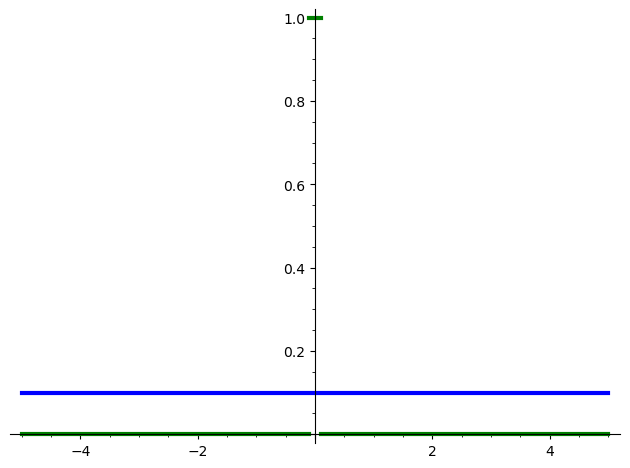
\includegraphics[width=0.5\textwidth]{graphics/lp_comparison}
\end{figure}

\begin{subsec}
It is worth contrasting the norms $L^{1}$ and $L^{\infty}$. $L^{1}$ only cares about the ``area under the graph''; a function $f$ whose graph is a narrow but very tall spike is tiny in $L^{1}$. Meanwhile $L^{\infty}$ only cares about ``height of the graph''; that same function $f$ would have an enormous $L^{\infty}$ norm.
On the other hand, a function which is very wide but shallow would be tiny in $L^{\infty}$ but huge in $L^{1}$.
See Figure \ref{Lp comparison figure}.
Later we will define $L^{p}$ norms which serve as a ``weighted average'' between the two extremes.
\end{subsec}

\begin{lemma}
The space $L^{1} \cap L^{\infty}$ of almost bounded integrable (equivalence classes of) functions is dense in $L^{1}$.
\end{lemma}
\begin{proof}
One has $\ISF \subseteq L^{1} \cap L^{\infty} \subseteq L^{1}$, but $\ISF$ is dense in $L^{1}$, so $L^{1} \cap L^{\infty}$ is as well.
\end{proof}

\begin{subsec}
How are the $L^{\infty}$ and $L^{1}$ norms related?
Well, if the measure of $X$ is finite, then the graph of the function cannot be ``too wide'', as our next lemma shows.
\end{subsec}

\begin{lemma}
If $\mu(X) < \infty$ then
\[||f||_{1} \leq \mu(X) ||f||_{\infty}.\]
\end{lemma}
\begin{proof}
We check
\[||f||_{1} \leq \int_{X} ||f(x)||~d\mu(x) \leq \int_{X} ||f||_{\infty} ~d\mu = ||f||_{\infty} \int_{X} ~d\mu = ||f||_{\infty} \mu(X).\]
Easy as that!
\end{proof}

\begin{subsec}
Conversely, if the graph of the function cannot be ``too skinny'', then we have the opposite bound.
To make this precise, we need the notion of a ``granular measure''.
\end{subsec}

\begin{definition}
A \dfn{granular measure} is a measure $\mu$ such that there is a $\delta > 0$ such that for every measurable set $E$, either $E = \emptyset$ or $|\mu|(E) \geq \delta$.
\end{definition}

\begin{subsec}
For example, counting measure is $\delta$-granular, with $\delta = 1$.
Another example is Lebesgue measure restricted to the $\sigma$-algebra generated by the intervals $[n, n+1]$, which is also $1$-granular.
\end{subsec}

\begin{lemma}
If $\mu$ is $\delta$-granular, then
\[||f||_{\infty} \leq \frac{||f||_{1}}{\delta}.\]
\end{lemma}
\begin{proof}
If $f = 0$ almost everywhere, then both sides of the claimed equation are $0$.
Otherwise, let $E_{n} = \{||f|| > ||f||_{\infty} - 1/n\}$; then $\mu(E_{n}) \geq \delta$ and $E_{n} \supseteq E_{n+1}$, so let $E = \bigcap_{n} E_{n}$; either $|\mu|(E_{n}) < \infty$ for some $n$ or $|\mu|(E_{n}) = \infty$ for all $n$.
In the latter case, there is an $n$ large enough that $||f||_{\infty} - 1/n > 0$ and
\[||f||_{1} \geq \int_{E_{n}} ||f(x)||_{B} ~d|\mu|(x) \geq (||f||_{\infty} - \frac{1}{n}) |\mu|(E) = \infty\]
and there is nothing to prove. Otherwise, $|\mu|(E) = \lim_{n} |\mu|(E_{n}) \geq \delta$ and
\[||f||_{1} \geq \int_{E} ||f(x)||~d|\mu|(x) \geq ||f||_{\infty} \delta,\]
proving the claim.
\end{proof}

\begin{figure}
\label{continuous function figure}
\caption{A typical continuous function on the compact set $[0, 1]$. Both the $L^1$ and $L^\infty$ norms are finite (and, in fact, are less than $36$).}
\centering 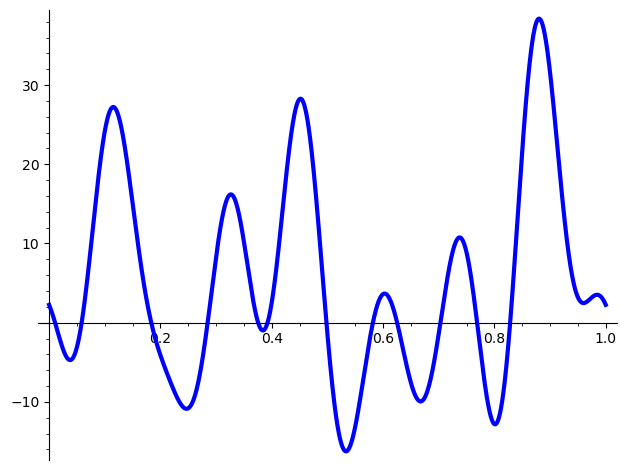
\includegraphics[width=0.5\textwidth]{graphics/typical_continuous}
\end{figure}

\begin{subsec}
Let us now show that for Radon measures, and in particular Lebesgue measure, continuous functions are integrable on compact sets, as in Figure \ref{continuous function figure}.
If the reader is unfamiliar with locally compact Hausdorff spaces, they may as usual take $X = \RR^{d}$ and $\mu$ Lebesgue measure.
\end{subsec}

\begin{definition}
Let $X$ be a locally compact Hausdorff space, and suppose that $\mu$ is a Radon measure on $X$.
A \dfn{locally integrable function} is a function $f$ such that for every compact set $K$, $f|K$ is an integrable function on $K$.
The space of locally integrable functions modulo null sets is denoted $L^{1}_{l}$.
A \dfn{almost locally bounded function} is a function $f$ such that for every compact set $K$, $f|K$ is almost bounded on $K$.
The space of almost locally bounded functions modulo null sets is denoted $L^{\infty}_{l}$.
\end{definition}

\begin{lemma}
Let $X$ be a locally compact Hausdorff space, and suppose that $\mu$ is a Radon measure on $X$.
Let $f$ be a continuous function; then $f \in L^{1}_{l} \cap L^{\infty}_{l}$.
\end{lemma}
\begin{proof}
First note that every continuous function is bounded on a compact set $K$.
Therefore $f \in L^{\infty}_{l}$, and since $\mu$ is Radon, $|\mu|(K) < \infty$; therefore
\[\int_{K} ||f(x)||~d|\mu|(x) \leq \sup_{x \in K} ||f(x)||\cdot |\mu|(K) < \infty.\]
Therefore $f \in L^{1}_{l}$.
\end{proof}

\begin{exercise}
Show that every set with Jordan content (see Exercise~\ref{Jordan content 1}) is Borel.
\end{exercise}

\section{Indefinite integrals}
In calculus, one defined the indefinite integral $g$ of a continuous function $f: [a, b] \to \RR$ by the relation
\[g(x) = \int_{a}^{x} f(t)~dt.\]
By the fundamental theorem of calculus, $g$ is differentiable and $g' = f$.
So we would like to define the indefinite integral of an arbitrary measurable function, and we would like it to have good regularity properties, but this is problematic; we used the order structure of $\RR$ to choose the interval $[a, x]$, but there is no such thing as an order on an arbitrary measure space, and there is no such thing as a differentiable function on an arbitrary measure space either.

But what if we thought of the indefinite integral as a function of the \emph{set} $[a, x]$ rather than the number $x$?
As it turns out, this will fix both problems, and also the pesky issue of needing to choose $a$ (the somewhat arbitrary choice of $a$ being the reason for the constant of integration that has caused calculus students so much grief).

\begin{subsec}
Throughout, let $X = (X, \Sigma, \mu)$ be a complete measured space, with $\mu$ valued in $(-\infty, \infty]$ or $\CC$, and $B$ a Banach space.
\end{subsec}

\begin{definition}
Let $f \in M$ and suppose that $\int f$ is defined. For every measurable set $E$, define
\[\nu(E) = \int_{E} f~d\mu.\]
We call $\nu$ the \dfn{indefinite integral} of $f$.
We also write $f = d\nu/d\mu$ and call $f$ the \dfn{Radon-Nikodym derivative} of $\nu$.
If $\nu$ is a measure which is an indefinite integral, we say that $\nu$ is \dfn{Radon-Nikodym differentiable}.
\end{definition}

\begin{subsec}
The hypothesis that $\int f$ is defined rules out the possibility that $\nu(E) = \infty - \infty$.
It is satisfied, for example, if $f \in L^{1}$ or $f \geq 0$.
\end{subsec}

\begin{lemma}
Let $f,g \in M$. Suppose that the indefinite integrals $\nu_{f},\nu_{g}$ of $f,g$ are defined. Then for every measurable set $E$,
\[||\nu_{f}(E) - \nu_{g}(E)||_{B} \leq ||f - g||_{1}.\]
\end{lemma}
\begin{proof}
One checks
\[||\nu_{f}(E) - \nu_{g}(E)||_{B} = \left|\left| \int_{E} f - g ~d\mu\right|\right| \leq ||f - g||_{1}\]
which proves the claim.
\end{proof}

\begin{theorem}
Suppose that $f \in L^{1}$, and $\nu$ is the indefinite integral of $f$. Then $\nu$ is a finite measure.
\end{theorem}
\begin{proof}
Finiteness follows from $f \in L^{1}$, so we just need to check that $\nu$ is countably additive.
We first check this when $f \in \ISF$. Indeed, if $f = b1_{E}$ is the canonical representation of $f$ and the $F_{j}$ are a sequence of disjoint measurable sets with union $F$, then
\[\nu(F) = b\mu\left(E \cap \bigcup_{j} F_{j}\right) = \sum_{j} b\mu(E \cap F_{j}) = \sum_{j} \nu(F_{j}).\]
Otherwise, $f$ is a linear combination of functions with canonical representation of the form $b1_{E}$ and the claim still follows.

Now if $f \in L^{1}$, then for every $\varepsilon > 0$ there is a $g \in \ISF$ such that $||f - g||_{1} < \varepsilon$; let $\rho$ be the indefinite integral of $g$. Then for every measurable set $E$, $||\nu(E) - \rho(E)||_{B} \leq ||f - g||_{1} < \varepsilon$.

If all but finitely many of the $F_{j}$ are empty, then there is an $N$ such that
\[\nu(F) = \int_{F} f ~d\mu = \sum_{j<N} \int_{F_{j}} f~d\mu = \sum_{j<N} \nu(F_{j}) = \sum_{j} \nu(F_{j}).\]
So it suffices to show that as $N \to \infty$, the partial sum $\sum_{j<N} \nu(F_{j})$ converges to $\nu(F)$.
Let $F^{N} = \bigcup_{j<N} F_{j}$, so $\nu(F^{N}) = \sum_{j<N} \nu(F_{j})$.

We already showed that $\rho$ is a measure, so if $N$ is large enough then for every $n > N$,
\[||\rho(F) - \rho(F^{N})||_{B} < \varepsilon.\]
In particular,
\begin{align*}
||\nu(F) - \nu(F^{N})||_{B} \leq ||\nu(F) - \rho(F)||_{B} + ||\rho(F) - \rho(F^{N})||_{B} + ||\rho(F^{N}) - \nu(F^{N})||_{B} < 3\varepsilon.
\end{align*}
This implies $\nu(F^{N}) \to \nu(F)$.
\end{proof}

Radon-Nikodym differentiable measures have a particularly easy-to-understand total variation.
\begin{theorem}
Let $\nu$ be a Radon-Nikodym differentiable measure. Then for any measurable set $E$,
\[|\nu|(E) = \int_{E} \left|\left|\frac{d\nu}{d\mu}(x)\right|\right|~d|\mu|(x).\]
\end{theorem}
\begin{proof}
Let $f = d\nu/d\mu$.

Suppose that $E$ is a measurable set and $E = \bigcup_{i} E_{i}$, a finite disjoint union. Then
\[\sum_{i} ||\nu(E_{i})|| = \sum_{i} \left|\left| \int_{E_{i}} f~d\mu\right|\right| \leq \int_{E} ||f(x)||~d\mu(x).\]
Taking the supremum over all such finite disjoint unions we see that $|\nu|(E) \leq \int_{E} ||f||$.

We first check the converse when $f \in \ISF$. Let $f = \sum_{i \leq k} b_{i} 1_{F_{i}}$ where the $F_{i}$ are disjoint.
Let $F = \bigcup_{i} F_{i}$.
Let us write $E \cap F_{i} = \bigcup_{j \leq n_{i}} G_{ij}$ where the $G_{ij}$ are disjoint. Then
\[|\nu|(E) \geq \sum_{i,j} ||\nu(G_{ij})||_{B} = \sum_{i,j} ||b_{i}||_{B} |\mu(G_{i,j})| = \sum_{i} ||b_{i}||_{B} \sum_{j} |\mu(G_{ij})|.\]
That is,
\[|\nu|(E) \geq \int_{E} ||f(x)|| ~d|\mu|(x).\]

In general, if $f,g \in L^{1}$ are the derivatives of $\nu,\lambda$ respectively, then
\[||\nu|(E) - |\lambda||(E) \leq |\nu - \lambda|(E) \leq \int_{E} ||(f - g)(x)||_{B} ~d|\mu|(x) \leq ||f - g||_{L^{1}},\]
by the reverse triangle inequality, Theorem~\ref{reverse triangle inequality}.
Now a straightforward approximation argument shows that the ISF case extends to all of $L^{1}$.
\end{proof}

\begin{definition}
A measure $\nu$ is \dfn{absolutely continuous} with respect to $\mu$ if for every $\varepsilon > 0$ there is $\delta > 0$ such that for every measurable set $E$, if $|\mu|(E) < \delta$, then $|\nu|(E) < \varepsilon$.
\end{definition}

\begin{theorem}\label{indefinite integral is abs cts}
For every $f \in L^{1}$, the indefinite integral of $f$ is absolutely continuous.
\end{theorem}
\begin{proof}
Let $\varepsilon > 0$ be given.
Since $\ISF \subseteq L^{1} \cap L^{\infty}$, there is $g \in L^{\infty}$ such that $||f - g||_{1} \leq \varepsilon/2$.
Suppose that $E$ is a measurable set such that $|\mu|(E) < \varepsilon/2||g||_{\infty}$. Then
\begin{align*}
\int_{E} ||f(x)|| ~d|\mu|(x) &\leq ||f - g||_{1} + \int_{E} ||g(x)|| ~d|\mu|(x) \\
&\leq ||f - g||_{1} + |\mu|(E)||g||_{\infty} \leq \varepsilon
\end{align*}
which completes the proof.
\end{proof}

\begin{subsec}
Later we will show the Radon-Nikodym theorem, which says that a measure $\nu$ is absolutely continuous iff every $\mu$-null set is automatically $\nu$-null, which happens iff $\nu$ is differentiable.
\end{subsec}


\section{Convergence theorems}
One of the cornerstone of calculus and its applications is the ability to interchange an integral with another sort of limit.
Unfortunately, this sort of manuever is not valid in general.

\begin{example}
Let $f_{n} = 1_{[n, n + 1]}$. Then $f_{n} \to 0$ pointwise but
\[\lim_{n \to \infty} \int_{-\infty}^{\infty} f_{n}(x) ~dx = 1.\]
\end{example}

\begin{subsec}
Roughly speaking, there are two settings in which it is acceptable to commute an integral with a limit.
For one, if all functions involved are ``dominated'' by some function in $L^{1}$, then it is usually safe to do so; one way to make this precise is the dominated convergence theorem.
\end{subsec}

\begin{theorem}[dominated convergence]
Let $f_{n} \in L^{1}(X \to B)$, and suppose that $f_{n} \to f$ almost pointwise. If there is a $g \in L^{1}(X \to [0, \infty))$ such that for every $n$ and almost every $x \in X$,
\[||f_{n}(x)|| \leq g(x),\]
then $f \in L^{1}(X \to B)$ and $f_{n} \to f$ in $L^{1}(X \to B)$.
\end{theorem}
\begin{proof}
By Lemma~\ref{L1 functions almost have finite carrier}, there is a measurable set $E$ with $|\mu|(E) < \infty$ such that
\[\int_{X \setminus E} g(x) ~d|\mu|(x) < \varepsilon.\]
Thus
\[\int_{X \setminus E} ||f_{n}(x) - f_{m}(x)||_{B} \leq 2\int_{X \setminus E} g(x) ~d|\mu|(x) < 2\varepsilon.\]
Let $\nu$ be the indefinite integral of $g$.
By Theorem~\ref{indefinite integral is abs cts}, there is $\delta > 0$ so small that if $|\mu|(G) < \delta$ then $|\nu|(G) < \varepsilon$.
Since $E$ has finite measure, Egorov's theorem implies that there is a measurable set $F \subseteq E$ such that $|\mu|(E \setminus F) < \delta$ and $f_{n} \to f$ in $L^{\infty}(F)$.
But then $|\nu|(E \setminus F) < \varepsilon$, and so
\[\int_{E \setminus F} ||f_{n} - f_{m}(x)||_{B} \leq 2\int_{E \setminus F} g(x) ~d|\mu|(x) = 2|\nu|(E \setminus F) < 2\varepsilon.\]
In particular, $\int_{X \setminus F} ||f_{n} - f_{m}||_{B} ~d|\mu| < 4\varepsilon$.
Since $F$ has finite measure and $f_{n} \to f$ in $L^{\infty}(F)$, $f_{n} \to f$ in $L^{1}(F)$ and so $(f_{n})$ is Cauchy in $L^{1}$; so choose $N$ so large that if $n,m \geq N$ then
\[||f_{n} - f_{m}||_{L^{1}(F)} < \varepsilon.\]
Then
\[||f_{n} - f_{m}||_{1} \leq ||f_{n} - f_{m}||_{L^{1}(F)} + \int_{X \setminus F} ||f_{n} - f_{m}||_{B} ~d|\mu| < 5\varepsilon\]
so $(f_{n})$ is Cauchy in $L^{1}$.
Since $f_{n} \to f$ almost pointwise, it follows that $f_{n} \to f$ in $L^{1}$.
\end{proof}

\begin{example}
We will compute
\[\lim_{n \to \infty} \int_{0}^{n} {\left(1 + \frac{x}{n}\right)}^{n} e^{-2x} ~dx.\]
First we compute
\[\lim_{n \to \infty} {\left(1 + \frac{x}{n}\right)}^{n} e^{-2x} = e^{x} e^{-2x} = e^{-x}.\]
Now, we have a pesky changing bound of integration, so we write
\[\lim_{n \to \infty} \int_{0}^{n} {\left(1 + \frac{x}{n}\right)}^{n} e^{-2x} ~dx = \lim_{n \to \infty} \int_{0}^{\infty} 1_{[0, n]}(x) {\left(1 + \frac{x}{n}\right)}^{n} e^{-2x} ~dx.\]
Since the integrand converges to $e^{-x}$, after finitely many $n$ (which are are allowed to discard, since we only care about the limiting behavior), we get
\[1_{[0, n]}{(x) \left(1 + \frac{x}{n}\right)}^{n} e^{-2x} \leq 2e^{-x}.\]
On the other hand,
\[\int_{0}^{\infty} e^{-x} ~dx = 1,\]
so $x \mapsto 2e^{-x}$ is in $L^{1}$ and by dominated convergence,
\[\lim_{n \to \infty} \int_{0}^{n} {\left(1 + \frac{x}{n}\right)}^{n} e^{-2x} ~dx = \int_{0}^{\infty} \lim_{n \to \infty} 1_{[0, n]}(x) {\left(1 + \frac{x}{n}\right)}^{n} e^{-2x} ~dx = \int_{0}^{\infty} e^{-x} ~dx = 1\]
as desired.
These sorts of problems are very common on preliminary exams for graduate students, so the reader should probably master them.
\end{example}

\begin{subsec}
The other situation in which it is acceptable to interchange an integral with a limit is when we can strongly use the order structure of $\RR$ in teh codomain.
So, we will need to restrict to the case when $B = [0, \infty)$ for the rest of the section, and thus formulate the so-called monotone convergence theorem.
\end{subsec}

TODO:\@ Monotone convergence

\begin{corollary}\label{positive summation}
Let $f_{n} \geq 0$ be nonnegative integrable functions and $\mu$ a nonnegative measure on $X$. Then
\[\int_{X} \sum_{n} f_{n}~d\mu = \sum_{n} \int_{X} f_{n}~d\mu.\]
\end{corollary}
\begin{proof}
The sequence of partial sums is increasing, so we can apply monotone convergence.
\end{proof}

\begin{corollary}
Let $f \geq 0$ be a nonnegative measurable function and $\mu$ a nonnegative measure. Then
\[\int_{X} f~d\mu = \sup_{s} \int_{X} s~d\mu\]
where the supremum is taken over all nonnegative $s \in \ISF(X \to [0, \infty))$.
\end{corollary}
\begin{proof}
We first show that there is a sequence of simple functions $\leq f$ converging to $f$ monotonically.
Fix $n$, and let $A_{n} = \{0, 1/n, 2/n, \dots, n - 2/n, n - 1/n, n\}$.
For each $y \in A_{n}$, let $E_{y}^{n} = f^{-1}([y, y + 1/n))$. Let
\[f_{n} = \sum_{y \in A_{n}} y1_{E_{y}^{n}}.\]
Now let $s_{n} = \max_{m \leq n} f_{m}$.
Then $s_{n}$ is simple and and $s_{n} \leq s_{n+1}$, and $s_{n} \to f$ almost everywhere.
So
\[\lim_{n \to \infty} \int_{X} s_{n}~d\mu = \int_{X} f~d\mu\]
by monotone convergence. Therefore
\[\int_{X} f~d\mu \leq \sup_{s} \int_{X} s~d\mu.\]
Monotonicity of the integral implies the other direction.
\end{proof}


\begin{exercise}
Let $f$ be a measurable $B$-valued function. Show that if there $g \in L^{1}(X \to [0, \infty))$ with $||f||_{B} \leq g$ almost everywhere, then $f \in L^{1}$.
\end{exercise}

\begin{exercise}
Suppose that $|\mu|(X) < \infty$ (for example, $\mu$ is a probability measure). Let $(f_{n})$ be a sequence of functions in $L^{\infty}$ such that there is $C > 0$ such that for every $n$, $||f_{n}||_{L^{\infty}} \leq C$.
Show that if $f_{n} \to f$ almost pointwise, then $f_{n} \to f$ in $L^{1}$.
\end{exercise}

\begin{exercise}
Consider the \dfn{gamma function}
\[\Gamma(z) = \int_{0}^{\infty} x^{z - 1} e^{-x} ~dx.\]
Show that $\Gamma$ is well-defined when $z > 0$ and is infinitely differentiable there. Then show that $\Gamma(n + 1) = n! = \prod_{1\le k\le n} k$ if $n \in \NN$.
\end{exercise}

\begin{exercise}
Show that
\[\lim_{n \to \infty} \int_{0}^{1} \frac{n^{3/2} x}{1 + n^{2} x^{2}} ~dx = 0.\]
\end{exercise}

\section{Product measures}
Previous our development of the Lebesgue measure has been totally one-dimensional: we have defined the measure of a measurable subset of the line $\RR$.
We would like to do the same for higher-dimensional spaces.

We first review the notion of a product set. Suppose that we are given sets $X_{\alpha}$, where $\alpha$ ranges over a set $A$.
The \dfn{Cartesian product} $\prod_{\alpha \in A} X_{\alpha}$ is by definition the set of maps $x: A \to \bigcup_{\alpha \in A} X_{\alpha}$ such that for every $a \in A$, $x(\alpha) \in X_{\alpha}$.
We usually write $x_{\alpha}$ or $\pi_{\alpha}(x)$ to mean $x_{\alpha}$. The maps
\[\pi_{\beta}: \prod_{\alpha \in A} X_{\alpha} \to X_{\beta}\]
are known as \dfn{canonical projection}s and the sets $X_{\alpha}$ are known as \dfn{factors}.

We mainly will be interested in the case when $A = \{1, \dots, n\}$ is a finite set, in which case we write $X_{1} \times \cdots X_{n}$ to mean the product of sets $X_{i}$, $i \in A$.
An element of $X_{1} \times \cdots \times X_{n}$ can be written as an $n$-tuple $(x_{1}, \dots, x_{n})$, where $x_{i} \in X_{i}$.
For example, $\RR^{n}$ is a product of $n$ copies of $\RR$, and its elements are $n$-tuples of real numbers.

\begin{lemma}
Suppose that $X_{\alpha}$ are nonempty sets. Then $\prod_{\alpha} X_{\alpha}$ is nonempty.
\end{lemma}
\begin{proof}
We first note that we can assume that the $X_{\alpha}$ are disjoint. Indeed, if they are not, we can replace them with
\[X_{\alpha}' = X_{\alpha} \times \{\alpha\}.\]
Then elements of $X_{\alpha}'$ are pairs $(x, \alpha)$ where $x \in X_{\alpha}$.
There is an obvious bijection $X_{\alpha} \to X_{\alpha}'$, $x \mapsto (x, \alpha)$, so we identify the two sets $X_{\alpha}$ and $X_{\alpha}'$.
Henceforth we replace $X_{\alpha}$ with $X_{\alpha}$ and hence assume the $X_{\alpha}$ are disjoint.

Define a map $f: \bigcup_{\alpha \in A} X_{\alpha} \to A$ by declaring that if $x \in X_{\alpha}$ then $f(x) = \alpha$.
Since the $X_{\alpha}$ are all nonempty, $f$ is surjective.
By the axiom of choice, Axiom~\ref{axiom of choice}, there is an injective map $g: A \to \bigcup_{\alpha \in A} X_{\alpha}$ such that $f \circ g$ is the identity, and so $g(\alpha) \in X_{\alpha}$.
Define an element $x$ of $X_{\alpha}$ by letting $x_{\alpha} = g(\alpha)$.
\end{proof}
If $A$ is \emph{finite} --- the case that is the most interesting to us --- then the use of the axiom of choice in the above argument is unnecessary (but otherwise it cannot be avoided, because if every product of nonempty sets is nonempty, then the axiom of choice is necessarily true).
The use of the axiom of choice in the above argument is a hint that infinite products may be rather ill-behaved in measure theory.

Having discussed Cartesian products of sets, we now move on to products of measurable spaces.
\begin{definition}
Let $(X_{\alpha}, \Sigma_{\alpha})$ be measurable spaces.
A \dfn{measurable rectangle} in $\prod_{\alpha} X_{\alpha}$ is a Cartesian product $\prod_{\alpha} Y_{\alpha}$, where $Y_{\alpha} \in \Sigma_{\alpha}$ and all but finitely many of the $Y_{\alpha}$ are equal to $X_{\alpha}$.
The set of measurable rectangles is denoted $\bigoplus_{\alpha} \Sigma_{\alpha}$.
\end{definition}

The measurable rectangles do not form a $\sigma$-algebra in general.
For example, in $\RR^{2}$, the diagonal $\{(x, x): x \in \RR\}$ is not a rectangle, but will be in the $\sigma$-algebra generated by the rectangles, as we will later show.

The rather awkward requirement that finitely many of the $Y_{\alpha}$ are equal to the $X_{\alpha}$ can be explained by the following lemma.

\begin{lemma}
Let $(X_{\alpha}, \Sigma_{\alpha})$ be measurable spaces.
Then $\bigoplus_{m} \Sigma_{m}$ is a semiring in $\prod_{m} X_{m}$.
\end{lemma}
\begin{proof}
Let $E, F$ be measurable rectangles.
Since all but finitely many of the $E_{\alpha}$ are $X_{\alpha}$, we can rename those $\alpha$ such that $E_{\alpha} \neq X_{\alpha}$ to be natural numbers.
That is, the only $E_{\alpha}$ which are not $X_{\alpha}$ will be called $E_{1}, \dots, E_{m}$.
Then if any unrenamed $\alpha$ has $F_{\alpha} \neq X_{\alpha}$, we can rename those $\alpha$ to $m+1, \dots, n$.
Thus, we can assume that
\[A = \{1, \dots, n\} \cup B\]
where for every $\beta \in B$, $E_{\beta} = F_{\beta} = X_{\beta}$.
One can then ignore the $E_{\beta}$ and $F_{\beta}$ entirely, and so assume that $B = \emptyset$.
Then, arguing by induction, one can assume that $n = 2$.
So assume that $E = E_{1} \times E_{2}$ and $F = F_{1} \times F_{2}$.

Now products commute with intersections, so $E \cap F$ is also a product of measurable sets, hence a measurable rectangle.
One similarly checks that
\[(E_{1} \times E_{2}) \setminus (F_{1} \times F_{2}) = (E_{1} \times (E_{2} \setminus F_{2})) \cup (E_{1} \setminus F_{1}) \times (E_{2} \cap F_{2}).\]
The above union is disjoint.
\end{proof}

Therefore it is reasonable to want to define a premeasure on $\bigoplus_{m} E_{m}$, which we do shortly.

\begin{definition}
Let $(X_{\alpha}, \Sigma_{\alpha})$ be measurable spaces, and let $X = \prod_{\alpha} X_{\alpha}$.
The \dfn{product $\sigma$-algebra} $\bigotimes_{\alpha} \Sigma_{\alpha}$ is the $\sigma$-algebra on $X$ generated by measurable rectangles in $X$.
We call $(X, \bigotimes_{\alpha} \Sigma_{\alpha})$ the \dfn{product measurable space} of the $(X_{\alpha}, \Sigma_{\alpha})$.
\end{definition}

Let $(\prod_{\alpha} X_{\alpha}, \bigotimes_{\alpha} \Sigma_{\alpha})$ be a product measurable space. We will usually just denote this space by $\prod_{\alpha} X_{\alpha}$, leaving $\bigotimes_{\alpha} \Sigma_{\alpha}$ understood, since usually $\bigotimes_{\alpha} \Sigma_{\alpha}$ is the only interesting $\sigma$-algebra on $\prod_{\alpha} X_{\alpha}$.

We leave it to the categorically-minded reader to check that the product measurable space satisfies the universal property of products, and leave everyone else to quizzically wonder what such a sentence means.
This is another sign that our definition of measurable space, with its bizarre clause that all but finitely many of the factors are trivial, is ``correct''.

We recall that a measure $\mu$ is complex-valued if for every measurable $E$, $\mu(E)$ is a complex number or $\infty$.
We will restrict to complex-valued measures because we need to be able to multiply the measures of sets.
Actually, if $\mu$ is complex-valued, then we can define its \dfn{complex conjugate} $\overline \mu$ by $\overline \mu(E) = \overline{\mu(E)}$.
Then we can define the \dfn{real part} $\Re \mu = (\mu + \overline \mu)/2$ and \dfn{imaginary part} $\Im \mu = (\mu - \overline \mu)/2i$.
Then $\mu = \Re \mu + i\Im \mu$.
Thus whenever we work with complex-valued measures, we can replace them with real-valued measures whenever necessary.
For a real-valued measure, we define $\mu_+ = (\mu + \mu)/2$ and $\mu_- = (\mu - \mu)/2$, thus $\mu_{\pm}$ are nonnegative measures and $\mu_+ - \mu_- = \mu$.
So, when working with products of measured spaces, we will state theorems that are for complex-valued measures, but then prove them for nonnegative measures, since every complex-valued measure can be written as a sum of nonnegative measures.

\begin{definition}
Let $(X_{1}, \Sigma_{1}, \mu_{1}), \dots, (X_{n}, \Sigma_{m}, \mu_{n})$ be measured spaces, where all the $\mu_{m}$ are complex-valued measures.
We define a function $\bigoplus_{m} \mu_{m} = \mu_{1} \oplus \cdots \oplus \mu_{n}$ on $\bigoplus_{m} \Sigma_{m}$ by
\[\left(\bigoplus_{m} \mu_{m}\right)(E) = \mu_{1}(E_{1})\mu_{2}(E_{2}) \cdots \mu_{n}(E_{n}).\]
We take the convention $0 \times \infty = 0$ whenever necessary.
\end{definition}

We note that if we have an \emph{infinite} collection of measured spaces $(X_{\alpha}, \Sigma_{\alpha}, \mu_{\alpha})$, $\alpha \in A$ it is reasonable to define $\bigoplus_{\alpha} \mu_{\alpha}$ whenever we can guarantee that the infinite product $\prod_{\alpha} \mu_{\alpha}(E_{\alpha})$ converges.
For example this happens if, for every $\alpha$, $\mu_{\alpha}$ is a probability measure.
However, this case can be rather tricky, due to the technicalities in the definition of a product of infinitely many measurable spaces.
We discuss this in more detail in Example~\ref{cantor measure}.

\begin{lemma}\label{product premeasure is a premeasure}
Let $(X_{1}, \Sigma_{1}, \mu_{1}), \dots, (X_{n}, \Sigma_{m}, \mu_{n})$ be measured spaces, where all the $\mu_{m}$ are complex-valued measures.
Then $\bigoplus_{m} \mu_{m}$ is a premeasure on $\bigoplus_{m} \Sigma_{m}$.
\end{lemma}
\begin{proof}
We must show that $\bigoplus_{m} \mu_{m}$ is $\sigma$-additive, and it suffices to check when $n = 2$, by induction.
By the usual reduction we can assume that the $\mu_{m}$ are nonnegative.
In that case we change notation and write $\eta = \mu \oplus \nu$, where $(X, \mu)$ and $(Y, \nu)$ are measured spaces.

Suppose that $E \times F$ is a rectangle which is a disjoint union of rectangles $E_{n} \times F_{n}$.
Then
\[1_{E}(x) 1_{F}(y) = 1_{E \times F}(x, y) = \sum_{n=1}^{\infty} 1_{E_{n} \times F_{n}}(x, y) = \sum_{n=1}^{\infty} 1_{E_{n}}(x) 1_{F_{n}}(y).\]
Therefore for any $x$,
\[1_{E}(x) \nu(F) = 1_{E}(x) \int_{Y} 1_{F}(y)~d\nu(y) = \int_{Y} \sum_{n=1}^{\infty} 1_{E_{n}}(x) 1_{F_{n}}(y) ~d\nu(y).\]
Thus by Corollary~\ref{positive summation},
\[1_{E}(x) \nu(F) = \sum_{n=1}^{\infty} 1_{E_{n}}(x) \int_{Y} 1_{F_{n}}(y)~d\nu(y) = \sum_{n=1}^{\infty} 1_{E_{n}}(x)\nu(F_{n}).\]
Applying Corollary~\ref{positive summation} again we see that
\[\eta(E \times F) = \mu(E) \nu(F) = \sum_{n=1}^{\infty} \mu(E_{n}) \nu(F_{n}) = \sum_{n=1}^{\infty} \eta(E_{n} \times F_{n}).\]
This is what we needed to prove.
\end{proof}

\begin{corollary}
Let $(X_{1}, \Sigma_{1}, \mu_{1}), \dots, (X_{n}, \Sigma_{m}, \mu_{n})$ be measured spaces, where all the $\mu_{m}$ are complex-valued measures.
Then $\bigoplus_{m} \mu_{m}$ extends to a measure on $\bigotimes_{m} \Sigma_{m}$, which is unique and $\sigma$-finite if the $\mu_{m}$ are all $\sigma$-finite.
\end{corollary}
\begin{proof}
Existence is obvious by Lemma~\ref{product premeasure is a premeasure} and the Carathéodory construction.
As for uniqueness, we use $\sigma$-finiteness of $\mu_{m}$ to find measurable sets $E_{m}^{k} \subseteq X_{m}$ such that $E_{m}^{k} \subseteq E_{m}^{k+1}$, $\bigcup_{k} E_{m}^{k} = X_{m}$, and $\mu_{m}(E_{m}^{k}) < \infty$.
Then $\prod_{m} E_{m}^{k} \subseteq \prod_{m} E_{m}^{k+1}$, $\bigoplus_{m} \mu_{m}(\prod_{m} E_{m}^{k}) = \prod_{m} \mu_{m}(E_{m}^{k}) < \infty$, and $\bigcup_{k} \prod_{m} E_{m}^{k} = \prod_{m} X_{m}$.
This implies that the extension of $\bigoplus_{m} \mu_{m}$ to a measure on $\bigotimes_{m} \Sigma_{m}$ is $\sigma$-finite and therefore unique.
\end{proof}

\begin{definition}
Let $(X_{1}, \Sigma_{1}, \mu_{1}), \dots, (X_{n}, \Sigma_{m}, \mu_{n})$ be measured spaces, where all the $\mu_{m}$ are complex-valued measures.
Let $\bigotimes_{m} \mu_{m} = \mu_{1} \otimes \cdots \mu_{n}$ be the extension of the premeasure $\bigoplus_{m} \mu_{m}$ to $\bigotimes_{m} \Sigma_{m}$.
We call $\bigotimes_{m} \mu_{m}$ the \dfn{product measure} of the $\mu_{m}$ and $(\prod_{m} X_{m}, \bigotimes_{m} \Sigma_{m}, \bigotimes_{m} \mu_{m})$ the \dfn{product measured space}.
\end{definition}

Let us give some examples of product measures.
We first consider the simplest example, which any reader who has played a children's card game is familiar with.

\begin{example}\label{card games}
Let $A = \{1, \dots, n\}$, equipped with the $\sigma$-algebra consisting of \emph{every} subset of $A$, and consider a function $\beta: A \to [0, 1]$ such that $\sum_{m=1}^{n} \beta(m) = 1$.
Then $\beta$ defines a probability measure $\mu$ by
\[\mu(\{a_{1}, \dots, a_{k}\}) = \sum_{j=1}^{k} \beta(a_{j}).\]
For example if $\beta = 1/n$, then $\mu$ is the \dfn{uniform probability measure} which sends every set $E$ to its cardinality divided by $n$.
If one has a set of $n$ cards, and the probability of drawing card $m$ is $\beta(m)$, then $\mu(E)$ is the probability of drawing a card in the set $E$.

Now we consider the Cartesian power $A^{\ell} = A \times \cdots \times A$ ($\ell$ factors).
Elements of $A^{\ell}$ are vectors of $\ell$ elements of $A$, and if $\mu^{\ell} = \bigotimes_{\ell} \mu$ is the product measure on $A^{\ell}$, then $\mu^{\ell}(E_{1} \times E_{2} \times \cdots \times E_{\ell})$ can be interpreted as the probability of first drawing a card in $E_{1} \subseteq A$, then in $E_{2} \subseteq A$, and so on, and then in $E_{\ell} \subseteq A$, with replacement.
In particular, if $E^{\ell} = E \times \cdots \times E$ is the Cartesian power of a set $E \subseteq A$, then $\mu^{\ell}(E^{\ell}) = \mu{(E)}^{\ell}$ is the probability of drawing a card in $E$ $\ell$ times in a row, with replacement.
\end{example}

\begin{example}\label{cantor measure}
Let $A, \beta$ be as in Example~\ref{card games}.
Now let us consider an infinitely long game, where one draws an infinite sequence of cards (the logicians would say that the player draws $\omega$ cards, because of TODO:Appendix) with replacement.
Let $A^{\omega}$ be the set of sequences with values in $A$, viewed as a measurable space by endowing it with the $\sigma$-algebra generated by the measurable rectangles.
By a cardinality argument similar to the one given in Lemma~\ref{Borel sigma algebra}, one can show that not every subset of $A^{\omega}$ is measurable.
On the other hand, the reader who is familiar with Cantor spaces (TODO:Appendix), and with the notion of the product of topological spaces (TODO:Appendix), will check that if we endow each copy of $A$ with the discrete topology (which is its unique Hausdorff topology) and then endow $A^{\omega}$ with the product topology, $A^{\omega}$ is Cantor, and every Borel set is measurable (and conversely, that every measurable set is Borel).

Since $\mu$ is probability, an infinite product of numbers $\mu(E_{n})$ will converge. Therefore if $E$ is a rectangle in $A^{\omega}$, and $\pi_{n}$ is the canonical projection onto the $n$th factor,
\[\mu^{\omega}(E) = \prod_{n} \mu(\pi_{n}(E))\]
is well-defined, and the reader can check (using the fact that for all $n$ large enough, $\mu(\pi_{n}(E))$ must be either $0$ or $1$ --- why?) that $\mu^{\omega}$ is a premeasure on the measurable rectangles, and hence a Borel probability measure.
In the case that $n = 2$ and $\mu$ is uniform (so $\beta = 1/2$), then we say that $\mu^{\omega}$ is the \dfn{standard Cantor measure}.
It is of essential importance in probability theory and logic, among other fields.
\end{example}

Example~\ref{cantor measure} motivates the idea that the product of Borel $\sigma$-algebras should be the Borel $\sigma$-algebra of the product spaces.
Unfortunately, this is not true in general.
We include the following example for the reader's amusement, but it is not terribly important and can be omitted.

\begin{example}
Let $\kappa$ be an uncountable cardinal as in TODO:Appendix, let $A = \{1, 2\}$ with its discrete topology, and let $X = A^{\kappa}$ be the Cartesian power, consisting of one factor of $A$ for each ordinal of cardinality less than $\kappa$. Let $\pi_{\alpha}$ be projection onto the $\alpha$th factor.
Let $\Delta$ be the diagonal, so $x \in \Delta$ iff there is a $y \in A$ for every $\alpha < \kappa$, $\pi_{\alpha}(x) = y$.

Since $X$ is a product of discrete (hence Hausdorff) spaces, $X$ is Hausdorff, so $\Delta$ is closed TODO:Appendix and hence Borel.
On the other hand, if $\Delta$ was measurable, then (as the set-theoretically minded reader can check) for all but countably many $\alpha$, $\pi_{\alpha}(\Delta) = A$, contradicting the fact that there are uncountably many $\alpha$ and $\pi_{\alpha}(\Delta) = \{y\}$.
\end{example}

The above example is highly pathological.
The below lemma covers most interesting cases.
We remind the reader that if $X_{m}$ are metric spaces with metrics $d_{m}$ then $\prod_{m} X_{m}$ can be given the metric
\begin{equation}\label{max metric}
d(x, y) = \max_{m} d_{m}(\pi_{m}(x), \pi_{m}(y)).
\end{equation}

\begin{lemma}\label{borel products}
Let $X_{1}, \dots, X_{n}$ be separable metric spaces.
Then the Borel $\sigma$-algebra on $\prod_{m} X_{m}$ is the product of the Borel $\sigma$-algebras on $X_{m}$.
\end{lemma}
\begin{proof}
By induction we can assume $n = 2$, and then change notation to write $X = X_{1}$, $Y = X_{2}$. We let $\mathcal B(Z)$ denote the Borel $\sigma$-algebra of the metric space $Z$.

By a \dfn{Borel cylinder} in $X \times Y$ we mean a set of the form $\pi_{X}^{-1}(E)$ or $\pi_{Y}^{-1}(F)$ where $E$ is Borel in $X$ and $F$ is Borel in $Y$.
We mean similarly for a \dfn{Borel cylinder}.
We leave it to the reader to check that $\mathcal B(X) \otimes \mathcal B(Y)$ is generated by the Borel cylinders.
Clearly every Borel cylinder is Borel, so this implies that every element of $\mathcal B(X) \otimes \mathcal B(Y)$ is Borel.
TODO:\@ Draw a picture of a cylinder.

Conversely, since $X, Y$ are separable there are countable dense subsets $E, F \subseteq X, Y$.
Then $E \times F$ is countable and dense in $X \times Y$.
Let $B(x, y, r)$ denote the ball of radius $r$ centered at $(x, y)$; then $B(x, y, r) = B_{X}(x, r) \times B_{Y}(y, r)$ if we are using the metric~\ref{max metric}. Here $B_{X}(x, r)$ is a ball in $X$ and similarly for $B_{Y}$.
Let $\mathcal S$ be the set of $B(x, y, r)$ with $(x, y) \in E \times F$ and $r \in \QQ$; then any open set in $X \times Y$ is a countable union of sets in $\mathcal S$ and so $\mathcal S$ generates $\mathcal B(X \times Y)$.
Therefore $\mathcal B(X \times Y) \subseteq \mathcal B(X) \otimes \mathcal B(Y)$.
\end{proof}

In the following section we use Lemma~\ref{borel products} to define the Lebesgue integral in general.

\section{The Lebesgue integral}
Let $\mu$ be a Stieltjes measure.
Then $\mu$ is a Borel measure on $\RR$, and by Lemma~\ref{borel products}, a product of $d$ copies of $\mu$ gives rise to a Borel measure on $\RR^{d}$.
We will mainly be interested in the case when $\mu$ is the Lebesgue measure.

\begin{definition}
Let $\mu$ be the Lebesgue measure on $\RR$.
The Borel measure $\mu^{d} = \bigotimes_{i=1}^{d} \mu$ on $\RR^{d}$ is called the \dfn{Lebesgue measure} on $\RR^{d}$.
If $f \in L^{1}(\RR^{d}, \mu^{d})$, we say that $f$ is \dfn{Lebesgue integrable} and call $\int f~d\mu^{d}$ the \dfn{Lebesgue integral} of $f$.
\end{definition}

If $d = 2$ then the Lebesgue measure of a rectangle, or indeed any of the classical shapes, is just its area.
Similarly if $d = 3$ then the Lebesgue measure of a rectangular prism, or any other classical shape, is just its volume.
Thus Lebesgue measure generalizes the basic notions of Euclidean geometry to arbitrary (Borel) subsets of $\RR^{d}$.

In general Lebesgue measure is so important that we usually refer to it implicitly.
For example, we will usually just write $\int f$ or $\int f(x) ~dx$ for the Lebesgue integral of $f$.

In this section we record the basic properties of the Lebesgue measure.

\begin{theorem}\label{lebesgue is radon 2}
The Lebesgue measure is a $\sigma$-finite Radon measure.
\end{theorem}
\begin{proof}
By induction on $d$. When $d = 1$ this is the content of Theorem~\ref{lebesgue is radon}.
Now $\mu^{d} = \mu^{d-1} \otimes \mu$, and we know that both $\mu^{d-1}$ and $\mu$ are Radon.

First we check local finiteness. By the Heine-Borel theorem every compact set is bounded and hence is contained in a compact rectangle in $\RR^{d}$, which is a product of a compact rectangle in $\RR^{d-1}$ and a compact interval, both of which have finite measure.
TODO:Draw a picture.
This makes $\sigma$-finiteness easy to prove, because ${[-n, n]}^{d}$ is a compact (hence finite measure) rectangle that grows to be all of $\RR^{d}$.

Now we check inner regularity on open rectangles.
An open rectangle $U$ in $\RR^{d}$ is a product of an open rectangle $U^{*} = \prod_{i<d} \pi_{i}(U)$ in $\RR^{d-1}$ and an open interval $\pi_{d}(U)$.
Now if $K$ is compact in $U$, then obviously $\mu(K) \leq \mu(U)$.
Conversely, for every $\varepsilon > 0$, we can find a compact interval $K_{d} \subset \pi_{d}(U)$ with $\mu^{d}(\pi_{d}(U) \setminus K_{d}) < \varepsilon$ and a compact rectangle $K^{*} \subset U^{*}$ with $\mu^{d}(U^{*} \setminus K^{*}) < \varepsilon$. So $K = K^{*} \times K^{d}$ also has $\mu^{d}(U \setminus K)$ arbitrarily small.

Every open set $U$ is a countable union of almost disjoint\footnote{in the sense that their intersection is Lebesgue null} open rectangles $U_{n}$, which can be approximated from within by compact sets $K_{n}^{m} \subset U_{n}$ with $\mu(U_{n} \setminus K_{n}^{m}) < \varepsilon 2^{-m}2^{-n}$. Then the $K_{n}^{n}$ are disjoint and $L_{n} = \bigcup_{m \leq n} K_{m}^{m}$ is compact.
Moreover if $\mu^{d}(U) = \infty$ then $\mu^{d}(L_{n}) \to \infty$; otherwise
\[\mu^{d}(U) = \sum_{n} \mu^{d}(U_{n}) \leq \sum_{n} \mu^{d}(K_{n}^{n}) + \frac{1}{2^{n}2^{n}} < \varepsilon + \mu^{d}(L_{n}) + \sum_{m > n} \mu^{d}(K_{m}^{m})\]
and
\[\sum_{m > n} \mu^{d}(K_{m}^{m}) \leq \sum_{m > n} \mu^{d}(U_{m}) < \varepsilon\]
if $n$ is large enough, since the sequence of $\mu^{d}(U_{m})$ is absolutely summable.
Therefore the $L_{n}$ approximate $U$ from within.

The proof of outer regularity is similar to the proof of inner regularity, and we leave it as an exercise.
The reader may wish to use ``half-open rectangles'' in the proof of outer regularity.
\end{proof}

\begin{theorem}\label{translation invariance in Rd}
If $A$ is Borel in $\RR^{d}$ and $x \in \RR^{d}$, then the translation $A + x$ has the same Lebesgue measure as $A$.
\end{theorem}
\begin{proof}
See Exercise~\ref{translation invariance exer}.
\end{proof}

\begin{theorem}
Let $f: [\alpha, \beta] \to \RR$ be a bounded Riemann integrable function and let $R$ be its Riemann integral. Then
\[\int_{\alpha^{\beta}} f(x)~dx = R.\]
\end{theorem}
\begin{proof}
The Riemann integral approximates $f$ from below by step functions $f_{n}$ on $[\alpha, \beta]$ which converge to $f$ pointwise, and $R$ is the limit of the $f_{n}$ as $n \to \infty$.
Since $f$ is a bounded function on a set of finite measure it is in $L^{1}$, and then dominated convergence implies that the Lebesgue integral is the limit of the integrals of the $f_{n}$.
\end{proof}

Thus, we really have generalized the familiar notion of integration that many students learn about in high school or their first year of undergraduate education.
We now prove that the integral of a function is the area under its graph.

\begin{theorem}
Let $f \in L^{1}(\RR^{d} \to [0, \infty))$.
Let $U = \{(x, y): x \in \RR^{d}, ~0 \leq y \leq f(x)\} \subset \RR^{d+1}$.
Then
\[\mu^{d+1}(U) = \int_{\RR^{d}} f(x)~dx.\]
\end{theorem}
\begin{proof}
All functions here are nonnegative (so that we do not have to talk about ``net signed area''), so by monotone convergence and continuity of measure, it suffices to check this for simple functions, and then by linearity it suffices to check this for an indicator function $f = 1_{A}$.
But this is obvious:
\begin{align*}U &= \{(x, y): x \in \RR^{d}, ~0 \leq y \leq f(x)\} \\&= \{(x, y): x \in A, ~0 \leq y \leq 1\} \cup \{(x, y): x \notin A, ~0 \leq y \leq 0\} \\&= (A \times [0, 1]) \cup (A^{c} \times \{0\}).\end{align*}
Since $\mu^{d+1}(A^{c} \times \{0\}) = 0$,
\[\mu^{d+1}(U) = \mu^{d+1}(A \times [0, 1]) = \mu^{d}(A) \mu^{1}([0, 1]) = \mu^{d}(A) = \int_{\RR^{d}} 1_{A}(x)~dx.\]
That proves the claim.
\end{proof}

Be aware, however, that there are Riemann integrable functions which are not Lebesgue integrable.
The reason is that, to avoid integrals of the form $\infty - \infty$, we demanded that Lebesgue integrals converge absolutely, while the Riemann integral is allowed to converge conditionally.
See Exercise~\ref{sinc} for an example of this phemonenon.

\begin{exercise}\label{translation invariance exer}
Prove Theorem~\ref{translation invariance in Rd}. (Hint: Use Theorem~\ref{translation invariance in R1}.)
\end{exercise}

\begin{exercise}\label{euclidean group}
The \dfn{euclidean group} is the group of invertible functions $\RR^{d} \to \RR^{d}$ generated by translations, rotations around the origin, and reflections. Equivalently, it is the group generated by translations and orthogonal linear maps.
An element of the euclidean group is called a \dfn{rigid motion}. Show that if $A$ is a rigid motion and $\mu$ denotes Lebesgue measure, then $A_{*}\mu = \mu$.
This generalizes Theorem~\ref{translation invariance in Rd}.
\end{exercise}

\begin{exercise}
Let $A: \RR^{d} \to \RR^{d}$ be an invertible linear map, $\mu$ Lebesgue measurable, and $E$ a Lebesgue measurable set. Show that $A_{*}\mu(E) = |\det A|\mu(E)$.
(Hint: Use Exercise~\ref{euclidean group} to show that without loss of generality, we may assume that $A$ is positive. Now use the spectral theorem.)
\end{exercise}

\begin{exercise}\label{sinc}
Define the \dfn{sampling function} $\sinc: \RR \to \RR$ by $\sinc x = \sin x/x$ for $x \neq 0$ and $\sinc 0 = 1$.
Let $F(r)$ be the Riemann integral of $\sinc$ on $[0, r]$. Show that $\lim_{r \to \infty} F(r)$ exists and is finite.
However, show that $\sinc$ is not Lebesgue integrable on $[0, \infty)$.
\end{exercise}

\section{Changing the order of integration}
In this section we prove the following extremely useful theorem.
We let $f(x, \cdot)$ denote the function $y \mapsto f(x, y)$ whenever $f$ is a function of two variables; similarly for $f(\cdot, y)$.
\begin{theorem}[Fubini]
Let $(X, \Sigma, \mu)$ and $(Y, \Gamma, \nu)$ be $\sigma$-finite complex-valued measured spaces.
Let $f: X \times Y \to \CC$ be a nonnegative $(\Sigma \otimes \Gamma)$-measurable function.
Then the following are equivalent:
\begin{enumerate}
\item $f \in L^{1}(X \times Y \to \CC, \mu \otimes \nu)$.
\item For almost every $x \in X$, $f(x, \cdot) \in L^{1}(Y \to \CC, \nu)$ and the function
\[x \mapsto \int_{Y} f(x, y)~d\nu(y)\]
is in $L^{1}(X \to \CC, \mu)$.
\item For almost every $y \in Y$, $f(\cdot, y) \in L^{1}(X \to \CC, \mu)$ and the function
\[y \mapsto \int_{X} f(x, y)~d\mu(x)\]
is in $L^{1}(Y \to \CC, \nu)$.
\end{enumerate}
Moreover,
\begin{equation}\label{change order of integration}
\int_{X \times Y} f~d(\mu \otimes \nu) = \int_{X} \int_{Y} f(x, y) ~d\mu(x)~d\nu(y) = \int_{Y} \int_{X} f(x, y) ~d\nu(y) ~d\mu(x).
\end{equation}
\end{theorem}
We will weaken the hypotheses on this theorem somewhat before the end of the section.
Because of (\ref{change order of integration}) we can \emph{define} the \dfn{double integral} by
\[\iint_{X \times Y} f ~d\mu ~d\nu = \int_{X \times Y} f~d(\mu \otimes \nu).\]
One similarly defines triple integrals, quadruple integrals, et cetra, by induction.
Indeed, the hypothesis that only two measure spaces are in play in the statement of Fubini's theorem can be completely done away with, by induction, and one can consider arbitrary finite products of measure spaces.
We will also do away with the hypothesis that $f$ is nonnegative, at the price of requiring that $f \in L^{1}$.
This is necessary to protect ourselves from our old enemy, $\infty - \infty$.
We \emph{cannot} do away with the $\sigma$-finite hypothesis, however TODO:show this.

TODO:\@ State the Banach space valued version.

Before we prove Fubini's theorem, let us record three of its many applications.
\begin{corollary}
Let ${(x_{i,j})}_{i,j=1}^{\infty}$ be absolutely summable, thus
\[\sum_{i=1}^{\infty} \sum_{j=1}^{\infty} |x_{i,j}| < \infty,\]
or nonnegative, thus for every $i,j$, $x_{i,j} \geq 0$. Then
\[\sum_{i=1}^{\infty} \sum_{j=1}^{\infty} x_{i,j} = \sum_{j=1}^{\infty} \sum_{i=1}^{\infty} x_{i,j}.\]
\end{corollary}
\begin{proof}
This is an immediate consequence of Fubini's theorem applied to counting measure.
\end{proof}

\begin{corollary}\label{Gaussian integral formula}
One has the \dfn{Gaussian integral formula}
\[\int_{-\infty}^{\infty} e^{-x^{2}} ~dx = \sqrt \pi.\]
\end{corollary}
\begin{proof}
We first note that
\[\int_{-\infty}^{\infty} e^{-x^{2}}~dx = \int_{-\infty}^{\infty} e^{-y^{2}}~dy\]
since all we have done is replace a dummy variable. Therefore it suffices to show that
\begin{equation}\label{gaussian integral squared}
\int_{-\infty}^{\infty} e^{-x^{2}}~dx \int_{-\infty}^{\infty} e^{-y^{2}}~dy = \pi.
\end{equation}
Clearly $x \mapsto e^{-x^{2}}$ is nonnegative, so by Fubini's theorem we can replace the product integral by a double integral:
\[\int_{-\infty}^{\infty} e^{-x^{2}}~dx \int_{-\infty}^{\infty} e^{-y^{2}}~dy = \iint_{\RR^{2}} e^{-(x^{2} + y^{2})}~dA(x, y).\]
Here $A$ (short for area) is Lebesgue measure on $\RR^{2}$.
Now $\{0\}$ is a null set so we can discard it, and the reader who recalls their calculus class will diligently check that $\RR^{2} \setminus \{0\} \cong \RR_+ \times [0, 2\pi)$ according to the map $(r \cos \theta, r \sin \theta) \mapsto (r, \theta)$, where the open half-line $\RR_+$ is given the Borel measure $\mu$ with
\[\mu(E) = \int_{E} r~dr\]
and $[0, 2\pi)$ is given Lebesgue measure. That is,
\[dA(r \cos \theta, r \sin \theta) = d\mu(r) ~d\theta = r~dr~d\theta.\]
To check this claim, one just needs to show that the Borel sets in $\RR^{2} \setminus \{0\}$ are generated by ``rectangles'' (which here are sectors $\{(r \cos \theta, r \sin \theta): r \in [r_{1}, r_{2}], ~\theta \in [\theta_{1}, \theta_{2}]\}$), and that for every such rectangle $R$, which we identify with the (plain old) rectangle $[r_{1}, r_{2}] \times [\theta_{1}, \theta_{2}]$, its area satisfies
\[A(R) = (\theta_{2} - \theta_{1})\int_{r_{1}}^{r_{2}} r~dr.\]
TODO:Draw a picture of a sector
Once the reader verifies this, they are entitled to apply Fubini's theorem again, and
\[\iint_{\RR^{2}} e^{-(x^{2} + y^{2})}~dA(x, y) = \int_{0}^{2\pi} \int_{0}^{\infty} re^{-r^{2}}~dr~d\theta = 2\pi \int_{0}^{\infty} re^{-r^{2}}~dr.\]
Now this is really just a calculus problem: if $s = r^{2}$ then $ds = 2r~dr$, and so one easily checks that
\[\int_{0}^{\infty} re^{-r^{2}}~dr = \frac{1}{2}.\]
Then (\ref{gaussian integral squared}) immediately follows.
\end{proof}

\begin{corollary}
Let $X,Y$ be independent random variables of type $\RR$. If $X,Y$ are in $L^{1}$, then $E(XY) = (EX)(EY)$, and if $X^{2}, Y^{2} \in L^{1}$, then $\Var(X+Y) = \Var X + \Var Y$.
\end{corollary}
\begin{proof}
Let $\mu_{X},\mu_{Y}$ be the distributions of $X,Y$.
Let $A = A_{1} \times A_{2} \subseteq \RR^{2}$ be a Borel rectangle.
Then
\[\mu_{X} \otimes \mu_{Y}(A) = \mu_{X}(A_{1}) \mu_{Y}(A_{2}) = P(X \in A_{1}) P(Y \in A_{2}) = P(X \in A_{1} \cap Y \in A_{2})\]
by independence. On the other hand, the random variable $(X, Y)$ of type $\RR^{2}$ has distribution
\[\nu(A) = P(X \in A_{1} \cap Y \in A_{2})\]
so $\nu = \mu_{X} \otimes \mu_{Y}$.
It follows that
\[E(|X||Y|) = \int_{\RR^{2}} \prod_{j=1}^{n} |x||y| ~d\nu(x, y) = \iint_{\RR^{2}} |x||y| ~d\mu_{X}(x)~d\mu_{Y}(y)\]
by Exercise~\ref{integrating a distribution} and Fubini's theorem. This integral simplifies to
\[\iint_{\RR^{2}} |x||y| ~d\mu_{X}(x)~d\mu_{Y}(y) = \int_{-\infty}^{\infty} |x| ~d\mu_{X}(x) \int_{-\infty}^{\infty} |y| ~d\mu_{Y}(y) = (E|X|)(E|Y|)\]
by Exercise~\ref{integrating a distribution}.
So by Fubini's theorem we can repeat the above argument with absolute values dropped and conclude $E(XY) = (EX)(EY)$.

Now set $X' = X - EX$, $Y' = Y - EY$. Then $X',Y'$ are independent and $EX' = EY' = 0$, so $E(X'Y') = 0$.
Thus
\begin{align*}\Var(X + Y) &= E({(X' + Y')}^{2}) = E({(X')}^{2}) + E({(Y')}^{2}) + 2E(X'Y') \\
&= \Var X' + \Var Y' = \Var X + \Var Y
\end{align*}
as desired.
\end{proof}

Monotone Classes

TODO:\@ Prove Fubini

\begin{exercise}[Cavalieri's principle]
Let $E \subseteq \RR^{2}$ be a measurable set, $\mu^{d}$ Lebesgue on $\RR^{d}$, and $E_{x} = \{y \in \RR: (x, y) \in E\}$.
Show that
\[\mu^{2}(E) = \int_{-\infty}^{\infty} \mu^{1}(E_{x})~dx\]
(so that, in particular, $x \mapsto \mu^{1}(E_{x})$ exists almost everywhere and is measurable).
\end{exercise}

\begin{exercise}
Let $f$ be the function $f(x, y) = y^{-2}$ for $x < y$ and $f(x, y) = x^{-2}$ for $y < x$.
Show that $f$ is defined almost everywhere and measurable, and the iterated integrals $\int_{0}^{1}\int_{0}^{1} f(x,y)~dx~dy$ and $\int_{0}^{1}\int_{0}^{1} f(x,y)~dy~dx$ are finite, but $f \notin L^{1}({[0, 1]}^{2})$.
What went wrong?
\end{exercise}

\begin{exercise}[weak law of large numbers]
Let $X_{n}$ be a countable sequence of iid random variables of type $\RR$.
Assume that $\Var X_{n}$ makes sense and $EX_{n} = 0$. Show that
\[\lim_{n \to \infty} \frac{1}{n} \sum_{j=1}^{n} X_{j} = 0\]
in probability using Chebyshev's inequality, Exercise~\ref{Chebyshev}.
\end{exercise}

\begin{exercise}[Stone-Weierstrass theorem for polynomials]
One form of the Stone-Weierstrass theorem is the statement that for every continuous function $f: [0, 1] \to \RR$, there exists a sequence of polynomials that converge to $f$ in $L^{\infty}$.
Surprisingly, this deterministic statement has a simple probabilistic proof, which we now outline.

Fix $x \in [0, 1]$.
Show that there is a probability space $(\Omega, P)$ which admits iid random variables $X_{j}$ with $P(X_{j} = 1) = x$ and $P(X_{j} = 0) = 1 - x$.
(Hint: One constructive way to do this is to say that $\Omega$ is the Cantor set $\prod_{j} \{0, 1\}$.)

Let $\overline X_{n} = \sum_{j \leq n} X_{j}/n$ be the average of the first $n$ random variables $X_{j}$ and show that $B_{n}(x) = E(f(\overline X_{n}))$ is a polynomial in $x$.
For every $\varepsilon > 0$ there is a $\delta > 0$, which does not depend on $x$, such that $|x - y| < \delta$ implies $|f(x) - f(y)| < \varepsilon$.
Conclude that
\[|B_{n}(x) - f(x)| \lesssim \varepsilon + P(|\overline X_{n} - x| > \delta)\]
where the constant is allowed to depend on $f$ but not $x$.
Use Chebyshev's inequality, Exercise~\ref{Chebyshev}, to conclude the proof.
\end{exercise}
